\documentclass[hide notes,intlimits]{beamer}

\mode<presentation>
{
  \usetheme[footline]{UAFshade}
  \setbeamercovered{transparent}
}
% frames are 128 millimeters by 96 millimeters
% load packages
\usepackage[english]{babel}
\usepackage[latin1]{inputenc}
\usepackage[T1]{fontenc}
\usepackage{amsmath,amssymb,wasysym}
\usepackage{lmodern}
\usepackage{movie15}
\usepackage{tikz}
\usetikzlibrary{shapes,arrows}


% Some useful commands (from MPL)
\newcommand{\s}[1]{\ensuremath{\,\text{#1}}}
\newcommand{\unit}[1]{\ensuremath{\,\text{#1}}}

\definecolor{dark red}{HTML}{E41A1C}
\definecolor{dark green}{HTML}{4DAF4A}
\definecolor{dark violet}{HTML}{984EA3}
\definecolor{dark blue}{HTML}{084594}
\definecolor{dark orange}{HTML}{FF7F00}
\definecolor{light blue}{HTML}{377EB8}
\definecolor{light red}{HTML}{FB9A99}
\definecolor{light violet}{HTML}{CAB2D6}

\setbeamercolor{boxed}{fg=black,bg=uaf yellow}


\graphicspath{{figures/}}

\usetikzlibrary{shadows}

\newenvironment{transbox}{%
  \begin{tikzpicture}
    \node[drop shadow,rounded corners,text width=\textwidth,fill=white, fill opacity=0.6,text opacity=1] \bgroup
  }{
    \egroup;\end{tikzpicture}} 

\newenvironment{transbox-tight}{%
  \begin{tikzpicture}
    \node[drop shadow,rounded corners,fill=uaf yellow, fill opacity=0.75,text opacity=1] \bgroup
  }{
    \egroup;\end{tikzpicture}} 


% title page
\title[] % (optional, use only with long paper titles)
{PISM (Parallel Ice Sheet Model)}
\subtitle{Current status and future plans}


\author[Khroulev] % (optional, use only with lots of authors)
{Constantine Khroulev, Ed Bueler, Andy Aschwanden}
% - Give the names in the same order as the appear in the paper.
% - Use the \inst{?} command only if the authors have different
% affiliation.
\institute{
University of Alaska Fairbanks
}

\date{CESM LIWG Meeting, February 2012}

\subject{PISM: Current status and future plans}

\begin{document}

\AtBeginSection[]{}


\setbeamertemplate{background canvas}
{
  \tikz{\node[inner sep=0pt,opacity=1.0] {\includegraphics[width=\paperwidth]{uaf_beamer_shade_bg}};}
} 

% insert titlepage
\begin{frame}
  \titlepage
\end{frame}

\setbeamertemplate{background canvas}
{
  % empty
}

\section{PISM in three slides}

\begin{frame}
  \frametitle{PISM in 3 slides (1 of 3)}
  \framesubtitle{User's point of view}
  \begin{columns}
    \begin{column}{50mm}
      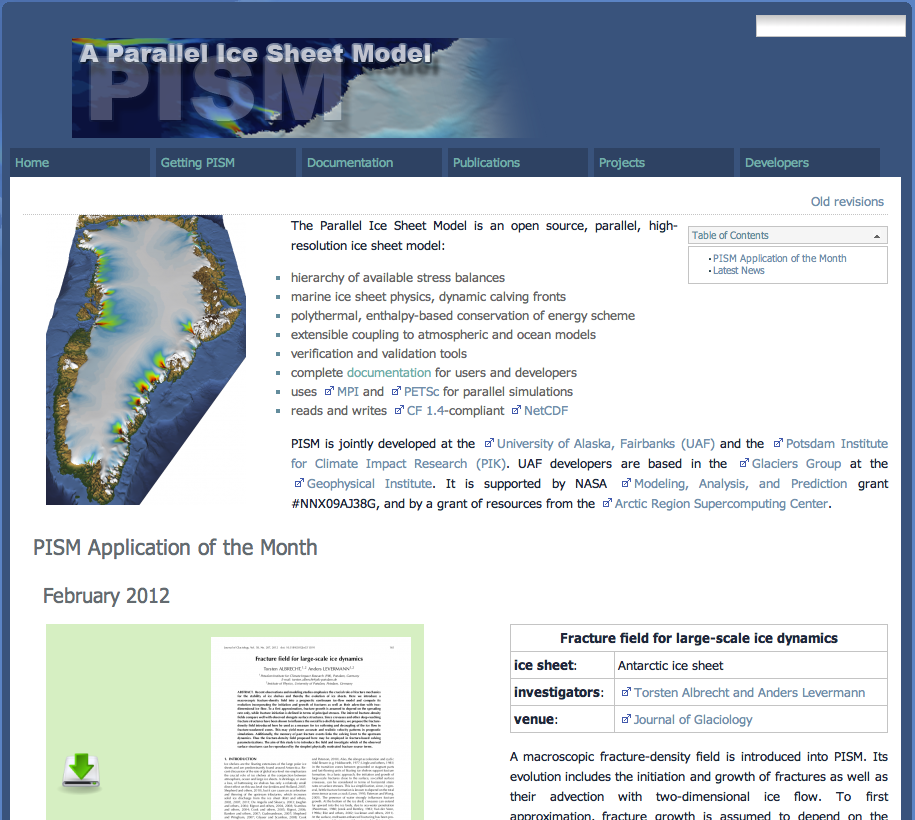
\includegraphics[width=50mm]{pismdocs.png}
    \end{column}
    \begin{column}{70mm}
      \begin{itemize}
      \item runs on Linux, Unix, and Mac OS X: from
        workstations to supercomputers
      \item stable versions are released once a year
      \item source code or a Debian/Ubuntu package
      \item website: \url{www.pism-docs.org}
      \item comprehensive User's Manual \mbox{(PDF, 120+ pages)}
      \item designed with usability in mind
      \end{itemize}
    \end{column}
  \end{columns}
\end{frame}

\begin{frame}
  \frametitle{PISM in 3 slides (2 of 3)}
  \framesubtitle{Power user's point of view}
  \begin{itemize}
  \item modular and extensible
  \item documented source code (\texttt{doxygen})
  \item everything is parallel (PETSc and MPI)
    \begin{itemize}
    \item whole Greenland at 2 km resolution
    \end{itemize}
  \item open source (GPL, hosted on \texttt{github.com})
  \item well-tested physics
    \begin{itemize}
    \item shallow hybrid
    \item enthalpy method
   \end{itemize}
  \end{itemize}
\end{frame}

\begin{frame}
  \frametitle{PISM in 3 slides (3 of 3)}
  \framesubtitle{Development point of view}
  \begin{itemize}
 \item supported by the NASA Modeling, Analysis and Prediction grant NNX09AJ38G
   through 2013
  \item since April 2011 PISM is developed jointly at UAF and the Potsdam
    Institute for Climate Impact Research (PIK)
  \end{itemize}
\end{frame}

\begin{frame}
  \frametitle{What do people do with PISM?}
 \begin{center}
    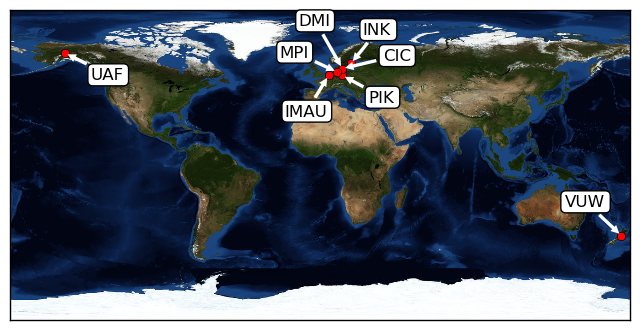
\includegraphics[width=120mm]{pism-users-map.png}
  \end{center}
\end{frame}

\section[Current status]{Current status (and applications)}

\begin{frame}
  \frametitle{People publish papers (with pretty pictures)}

  During the past year \emph{nine} PISM-related papers were published (or are about to
  appear):

  \begin{itemize}
  \item two papers by PISM users outside of UAF and PIK
    \begin{itemize}
    \item \textbf{Solgaard et al} (2011) \emph{Snapshots of
        the Greenland ice sheet configuration in the Pliocene to early
        Pleistocene}
    \item \textbf{van Pelt et al} (2012) \emph{Numerical
        simulations of cyclic behaviour in the Parallel Ice Sheet Model
        (PISM)}
    \end{itemize}
  \item six papers from the PIK group
    \begin{itemize}
    \item one description paper
    \item three modeling
    \item two applications
    \end{itemize}
  \item \textbf{Aschwanden et al} (2012) \emph{An enthalpy
      formulation for glaciers and ice sheets}
  \end{itemize}

\end{frame}

\begin{frame}
  \frametitle{We feature one project a month}
  \begin{center}
    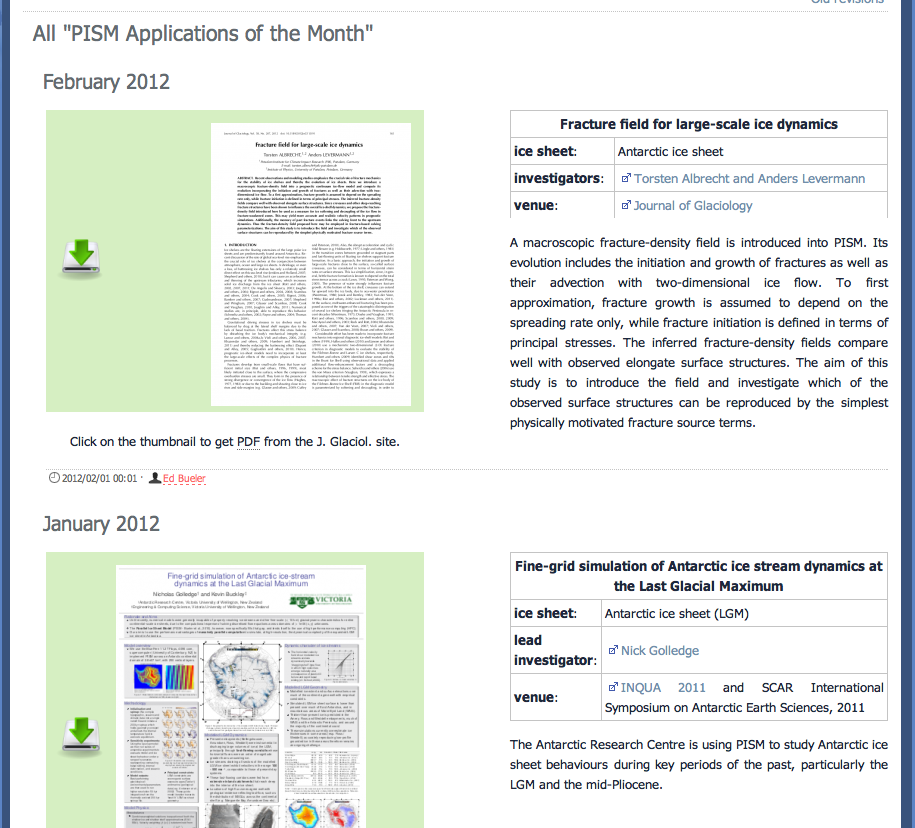
\includegraphics[height=0.75\textheight]{application-of-the-month.png}
  \end{center}
\end{frame}

\begin{frame}
  \frametitle{PISM-PIK merge}
  \framesubtitle{Subgrid-scale motion of the calving front}
  \begin{columns}
    \begin{column}{60mm}
      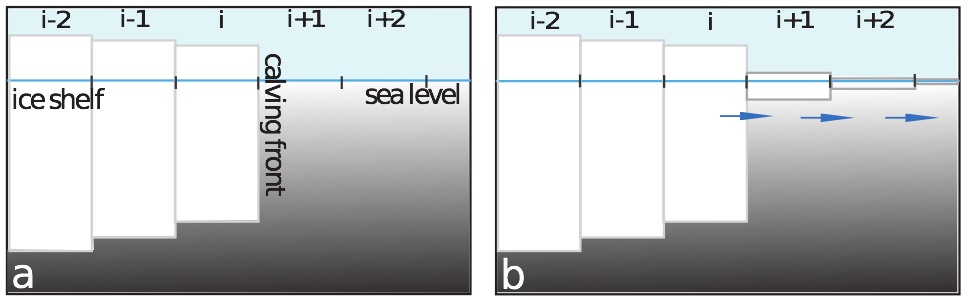
\includegraphics[width=60mm]{part-grid-scheme-1.png}\\
      \rule{0pt}{5mm}\\
      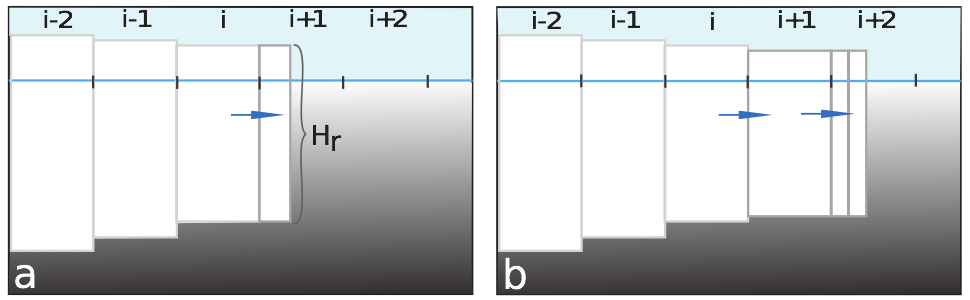
\includegraphics[width=60mm]{part-grid-scheme-2.png}\\
   \end{column}
    \begin{column}{60mm}
      \begin{itemize}
      \item avoids artificial thinning
      \item better modeling of the location of the front
      \item allows for advancing shelves
      \end{itemize}
   \end{column}
  \end{columns}
   \begin{flushleft}
      \tiny \textbf{Albrecht et al} (2011)
      \emph{Parameterization for subgrid-scale motion of ice-shelf calving
        fronts}. The Cryosphere 5 pp. 35--44.
   \end{flushleft}
\end{frame}

\begin{frame}
  \frametitle{PISM-PIK merge}
  \framesubtitle{First-order calving law}
  \begin{columns}
    \begin{column}{50mm}
      \begin{center}
        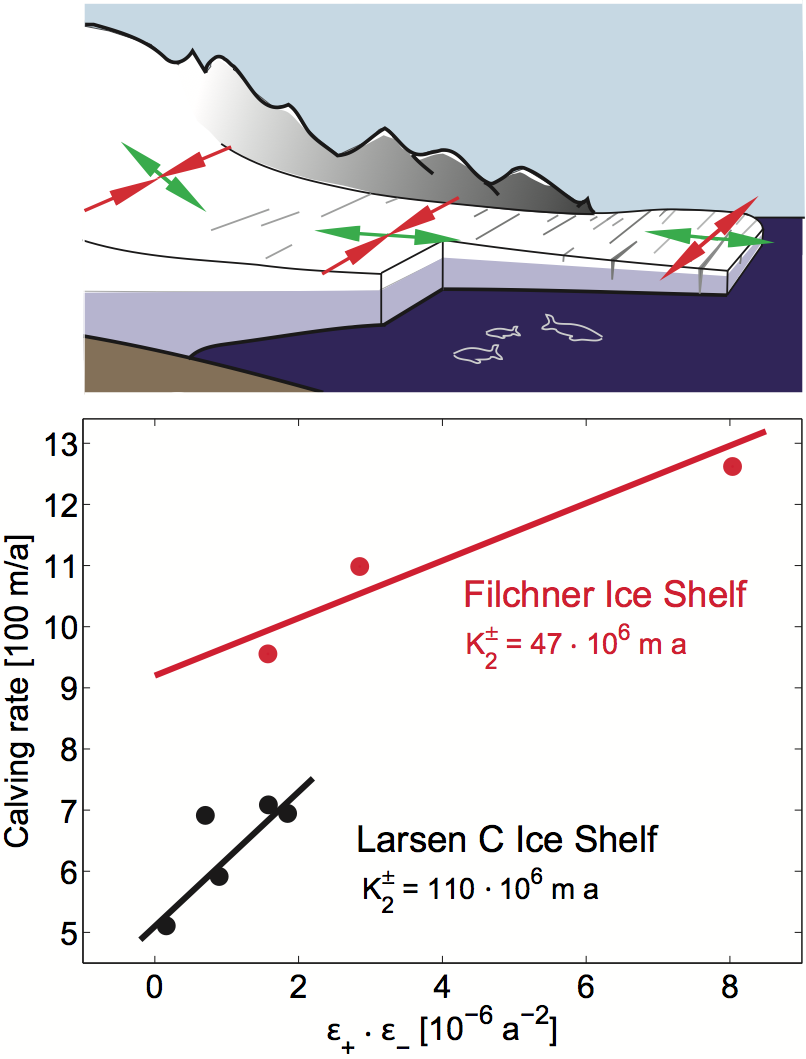
\includegraphics[height=0.6\textheight]{calving-law.png}
      \end{center}
    \end{column}
    \begin{column}{70mm}
      \begin{itemize}
      \item calving rate proportional to spreading rates in both
        eigen-directions:
        $$C = K_{2}^{\pm} \cdot \dot \epsilon_{+} \cdot \dot \epsilon_{-}$$
      \item has one scalar parameter
      \item allows for ice shelf retreat
      \end{itemize}
    \end{column}
  \end{columns}
  \begin{flushleft}
    \tiny \textbf{Levermann et al} (2011) \emph{Kinematic
      first-order calving law implies potential for abrupt ice-shelf
      retreat}. The Cryosphere Discussions 5 (5) pp. 2699--2722.
 \end{flushleft}
\end{frame}

\begin{frame}
  \frametitle{PIK application}
  \framesubtitle{Dynamic equilibrium simulation of the Antarctic ice sheet}

  \begin{center}
    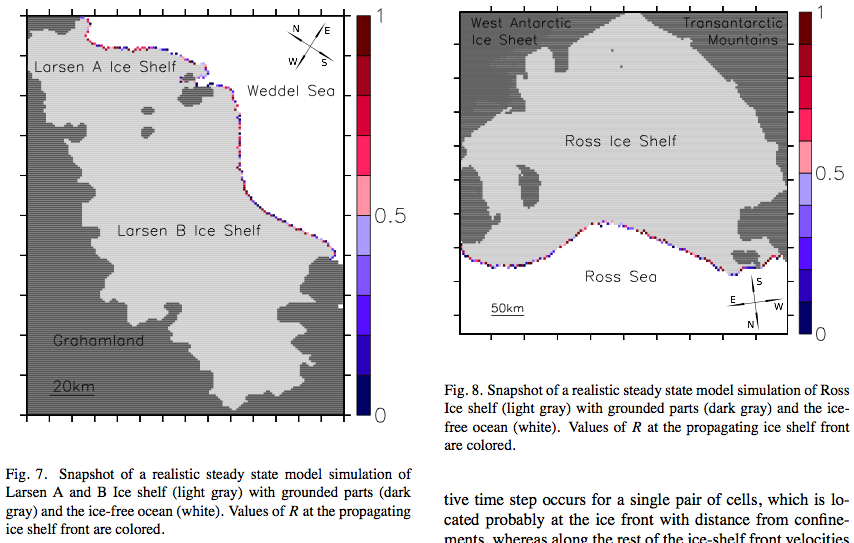
\includegraphics[height=0.7\textheight]{moving-calving-front.png}
  \end{center}
  \begin{flushleft}
    \tiny \textbf{Martin et al} (2011) \emph{The
        Potsdam Parallel Ice Sheet Model (PISM-PIK) Part 2: Dynamic
        equilibrium simulation of the Antarctic ice sheet}. The Cryosphere 5
      pp. 727--740.
  \end{flushleft}
\end{frame}

\begin{frame}
  \frametitle{PIK project}
  \framesubtitle{Fracture field for large-scale ice dynamics}
  \begin{center}
    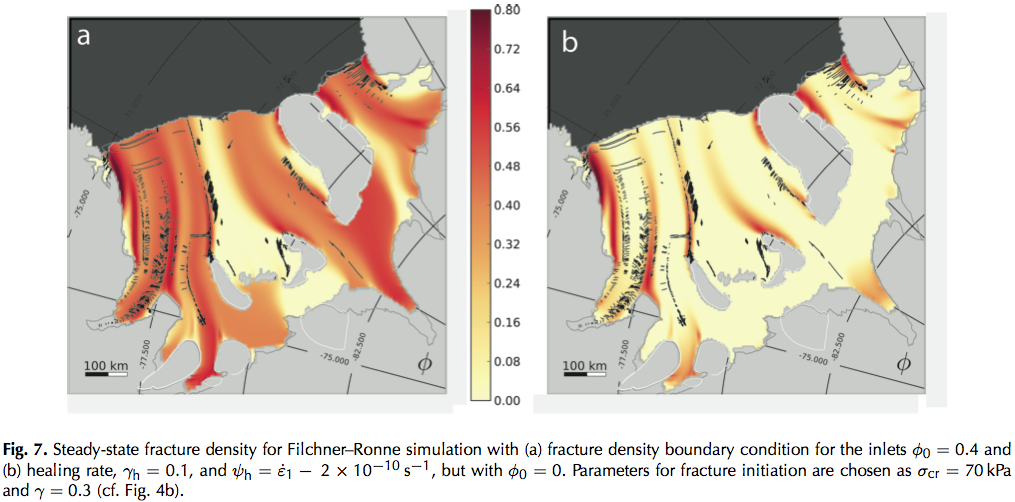
\includegraphics[width=0.9\textwidth]{fracture-density.png}
  \end{center}

  \begin{center}
    step toward fracture-based calving
  \end{center}

  \begin{flushleft}
    \tiny \textbf{Albrecht et al} (2012) \emph{Fracture field for
      large-scale ice dynamics}. Journal of Glaciology 58 (207) pp. 165--176.
 \end{flushleft}
\end{frame}

\begin{frame}
  \frametitle{UAF project}
  \framesubtitle{Enthalpy model}

  \begin{center}
    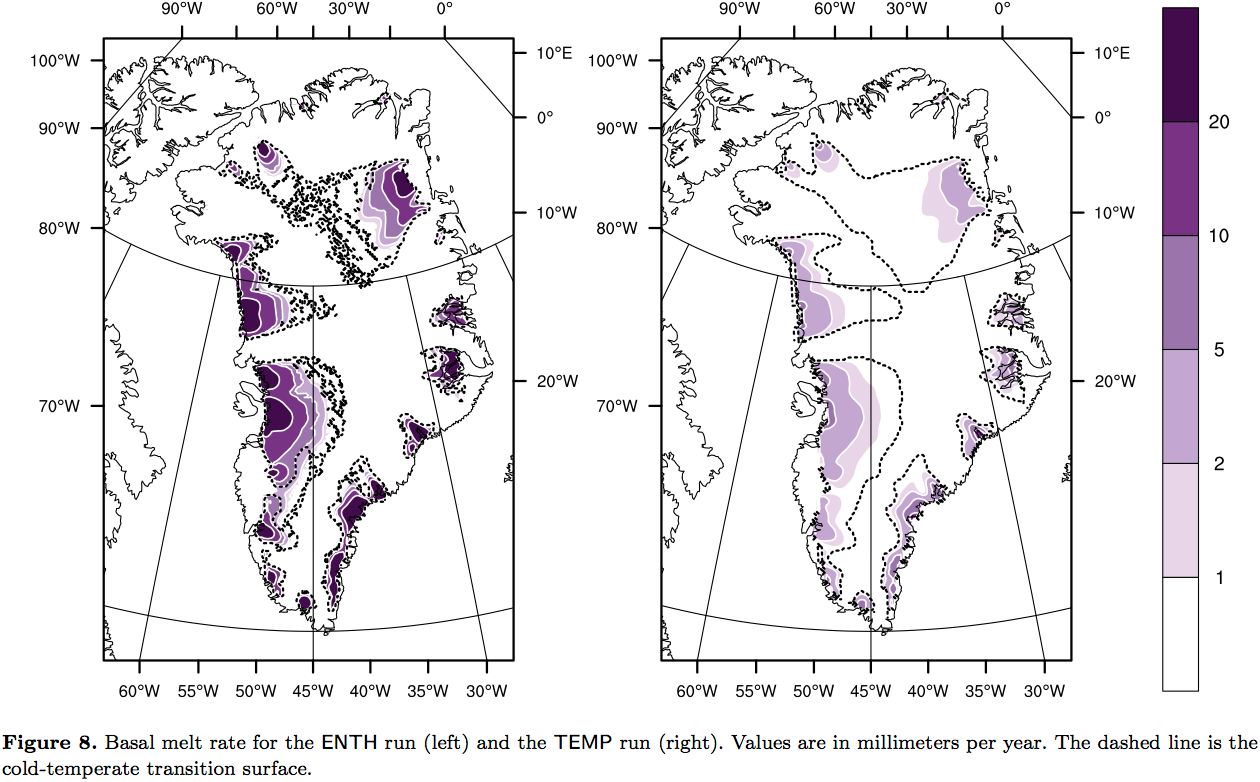
\includegraphics[height=0.7\textheight]{enthalpy-model.png}
  \end{center}

  \begin{flushleft}
  \tiny \textbf{Aschwanden et al} (2012) \emph{An enthalpy
      formulation for glaciers and ice sheets}. Journal of Glaciology, to
    appear
 \end{flushleft}
\end{frame}

\begin{frame}
  \frametitle{UAF project}
  \framesubtitle{PISM as a regional model}
  \begin{center}
    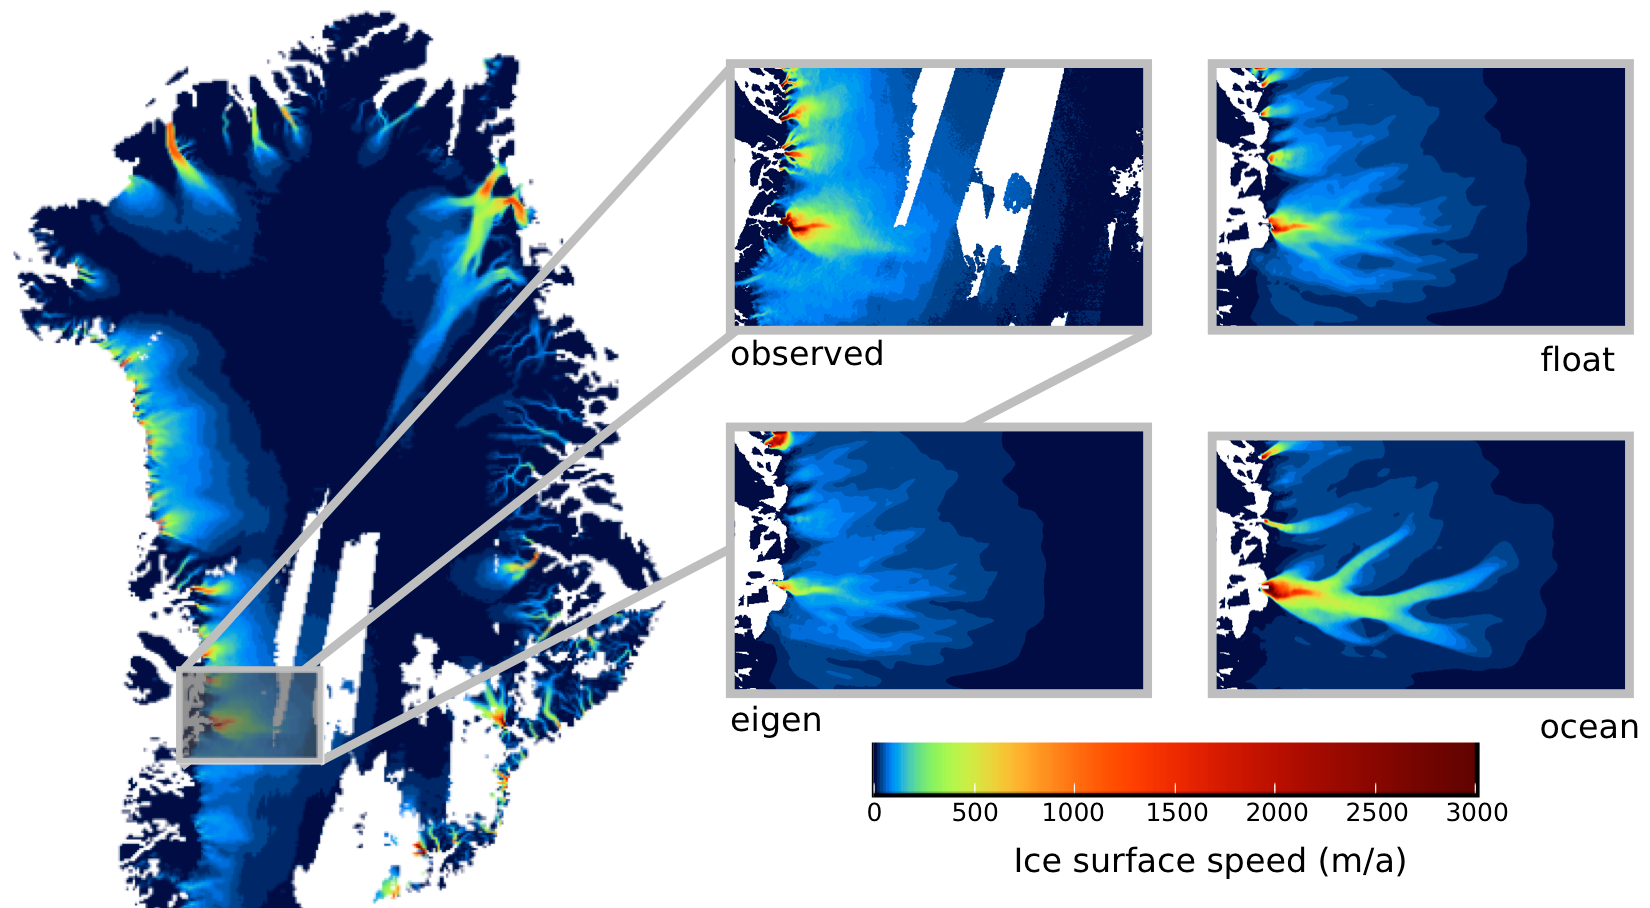
\includegraphics[width=0.95\textwidth]{csurf-regional.png}
  \end{center}
  \begin{flushleft}
    \tiny \textbf{Daniella DellaGiustina} (2011), \emph{Regional modeling of
      Greenland's outlet glaciers with the Parallel Ice Sheet Model}, M.S.
    Computational Physics thesis, UAF
  \end{flushleft}
\end{frame}

\begin{frame}
  \frametitle{UAF project}
  \framesubtitle{Validation using InSAR surface speed}
  \begin{columns}
    \begin{column}{90mm}
    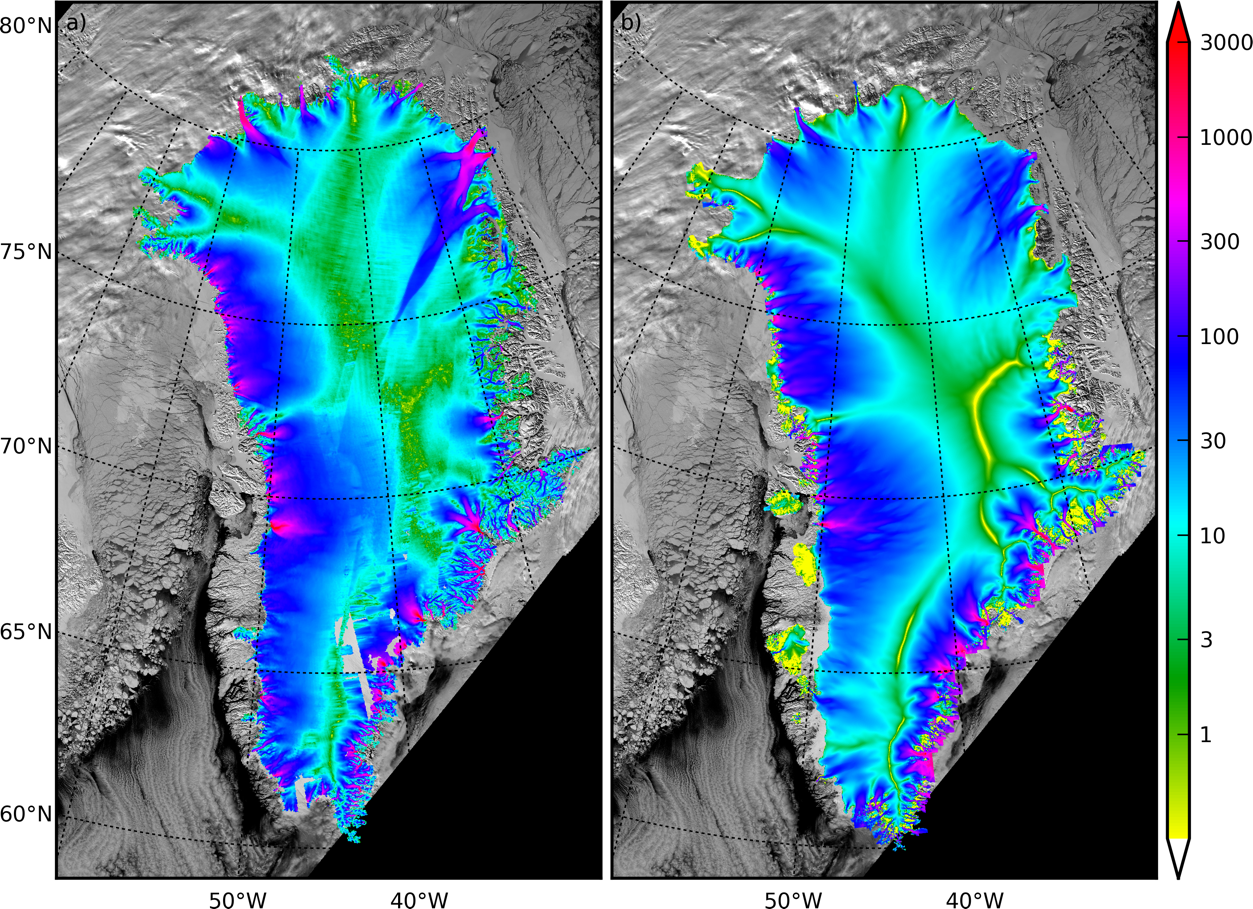
\includegraphics[width=90mm]{csurf-insar-pism-hhcmb.png}
    \begin{center}
       \tiny \textbf{Left:} InSAR surface speed in meters per year (Joughin, 2010)\\
        \textbf{Right:} PISM simulated surface speed
   \end{center}
   \end{column}

    \begin{column}{35mm}
      \begin{itemize}
      \item no inversion
      \item small number of parameters
      \item constant climate spin-up
      \item 2km grid
      \item Aschwanden et al, in prep.
      \end{itemize}
    \end{column}
  \end{columns}

\end{frame}

\section{Future plans}

\begin{frame}
  \frametitle{Future plans}
  \begin{itemize}
  \item inverse modeling (lead by David Maxwell and Marijke Habermann)
    \begin{itemize}
    \item uses new tools (written in Python)
    \item shares code with PISM
    \item well under way
    \end{itemize}
  \item basal hydrology model (Ed Bueler and Ward van Pelt)
  \item Blatter stress balance solver$^{*}$
  \item better coupling
  \item better transport/advection algorithm
  \end{itemize}

 \begin{flushleft}
   \tiny
    $^{*}$ See \textbf{Brown et al} (2011)
    \emph{Achieving textbook multigrid efficiency for hydrostatic ice sheet
      flow}, submitted to SIAM J. Scientific Computing.
  \end{flushleft}
\end{frame}


\end{document}

% LocalWords: Debian Ubuntu pismdocs Levermann Winkelmann Martin Aschwanden Bueler parameterization subgrid PIK png Ahmadia PDF pdf doxygen PETSc MPI GPL github UAF NNX AJ Cryosphere Solgaard Reeh Oerlemans polythermal InSAR Joughin Blatter DellaGiustina Marijke Habermann advection multigrid eigen